\documentclass{scrreprt}
\usepackage{listings}
\usepackage{underscore}
\usepackage{graphicx}
\usepackage[bookmarks=true]{hyperref}
\usepackage[utf8]{inputenc}
\usepackage[english]{babel}
\usepackage{fancyhdr}
\usepackage{emptypage}
\usepackage{lipsum}
\usepackage{appendix}
\usepackage{array}
\usepackage{amsmath}

\hypersetup{
    bookmarks=false,    % show bookmarks bar?
    pdftitle={Software Requirement Specification},    % title
    pdfauthor={Jean-Philippe Eisenbarth},                     % author
    pdfsubject={TeX and LaTeX},                        % subject of the document
    pdfkeywords={TeX, LaTeX, graphics, images}, % list of keywords
    colorlinks=true,       % false: boxed links; true: colored links
    linkcolor=black,       % color of internal links
    citecolor=black,       % color of links to bibliography
    filecolor=black,        % color of file links
    urlcolor=purple,        % color of external links
    linktoc=page            % only page is linked
}%
\def\myversion{1.0 }
\date{}
%\title
\usepackage{hyperref}
\begin{document}
\thispagestyle{empty}
\pagenumbering{roman}
\begin{flushright}
    \rule{16cm}{5pt}\vskip1cm
    \begin{bfseries}
        \Huge\textbf{SOFTWARE REQUIREMENTS\\ SPECIFICATION}\\
        \vspace{1cm}
        for\\
        \vspace{1cm}
        Attendance Application\\
        \vspace{1cm}
        \LARGE{Version \myversion approved}\\
        \vspace{1cm}
        \begin{align*}
        \text{Prepared by : } 
        &\text{1. Sanskar Mittal} &\text{(21CS10057)}\\
        &\text{2. Yash Sirvi} &\text{(21CS10083)}\\
        &\text{3. Ashwin Prasanth} &\text{(21CS10009)}
        \end{align*}

        \vspace{1cm}
        Submitted in partial \\fulfillment of the requirements of \\CS29202 Software Engineering Lab\\
        \vspace{1cm}
        \today\\
    \end{bfseries}
\end{flushright}
\renewcommand*\contentsname{Table of Contents}


\tableofcontents
\addcontentsline{toc}{chapter}{Table of Contents}

\newcommand{\addappendix}{%
  \chapter*{\appendixname}% start the appendix
  \addcontentsline{toc}{chapter}{\appendixname}% add it to the toc
  \counterwithin*{figure}{section}% optional, if you want to reset the figure counter
  %\stepcounter{section}% reset counters related to section
  \renewcommand{\thesection}{A}% we want A
  \renewcommand{\thefigure}%{\thesection.\arabic{figure}}% optional
}

\chapter*{Revision History}
\addcontentsline{toc}{chapter}{Revision History}

\begin{center}
\begin{tabular}{ | c | c | c | c | } 
  \hline
  Name & Date & Reason for changes & Version \\
  \hline\hline
  cell1 dummy text & cell6 & cell 7 & cell 8\\ 
  \hline
  cell9 & cell10 & cell 11 & cell 12\\ 
  \hline
\end{tabular}
\end{center}

\pagestyle{fancy}
\fancyhead{} % clear all header fields
\fancyhead[LO,LE]{\textbf{Software Requirements Specification for Attendance Application}}

\chapter{Introduction}
\pagenumbering{arabic}
\setcounter{page}{4}
\section{Purpose}
This is very much difficult to maintain all the data of a course as a hard copy. Any data can be changed, deleted, added at any time. Such as - A new teacher can be assigned for a course, he also can be changed ; And so many student are getting admitted every semester. So, "IICT WEBSITE" is the solution. "IICT WEBSITE" is a official website based on marking and resulting system of IICT authorized. The main concept of "IICT WEBSITE" is to devitalized PGD, MIT courses, their students and teachers data maintenance. 

\section{Intended Audience and Reading Suggestions}
This SRS is for developers, project managers, users and testers. Further the discussion will provide all the internal, external, functional and also non-functional informations about "IICT WEBSITE".

\section{Project Scope}
"IICT WEBSITE" creates a space for Director, Teachers, Students and Office Staffs for maintaining particular programs like - PGD, MIT. 
\newline
After getting admitted to a programs a student has been given a registration number, by using which he/she can inter from-fill-up page. It will take his/her personal informations, admitted fee imformations.He will be added as a student of that particuler programs after completing his/her payment process. After that he/she can select course of the program and then pay the fee for that. Student profile will contain all his personal informations, past results, recent result and notifications.
\newline
Office staff only post result publicly and also notice. But off course with the permission of Director.  
\newline
Directors' main work is to assign teachers to the courses they will take, create teachers profile and approve mark-sheet. He can move a teacher from one course to another. He also can be a teacher and can also can take the courses and perform all the functionality of teacher like- marking papers. He can also directly post notice to the website, teachers and also students.
\newline
Teachers' account are created by director. They (Teachers) entry marks of the students, can view all the marks of the students and change it after submitted it to the director. Every student of that particular course will be under the teacher who is assigned to that course. 
\newline
\begin{figure}
    \centering
    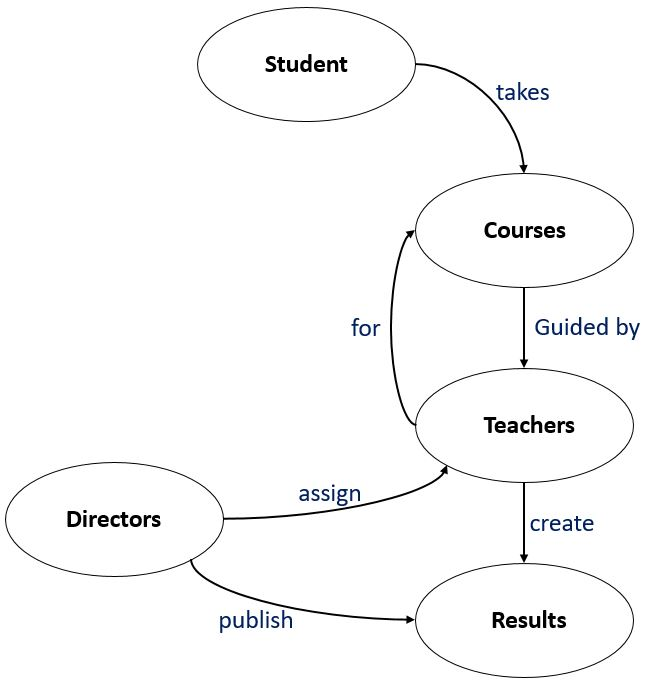
\includegraphics[width=10cm]{1.JPG}
    \caption{Entire work-flow}
    \label{fig:IICT WEBSITE}
\end{figure}
\newline
Figure 1.1 (Entire work-flow) is the overview of the project. Connection of all the entities are dependable to each others.  This gives the simple idea about the functional activities of the project. 
\newline
Student cycle, In the Figure 1.1 "Student" takes "Courses" ; "Courses" is guided by "Teachers"; "Teachers" creates "Results". 
\newline
Teacher cycle, In the Figure 1.1 "Director" assign "Teachers"; "Teachers" for particular "Courses"; "Director" publish "Results".
\newline
So, every entity is vary much interactive with each other.


\chapter{Overall Description}

\section{Product Perspective}
"IICT WEBSITE" is the replacement of the manual hard copy result process. The data have been stored in the hard file or papers, this website will store all of those in the website. Main goal of this project is to minimize the work and maximize the result of this result processing system.

\section{User Classes and Characteristics}
"IICT WEBSITE" has basically 4 types of users. 
\begin{itemize}
  \item Teachers
    \begin{itemize}
        \item Director
        \item Course Teacher
    \end{itemize}
  \item Students
  \item Official Staff
\end{itemize}
Teacher has 2 types - Director defines the course teachers who will take the courses. Student fulfill all the requirements like- fees, informations can take advantages of the website. 
\begin{figure}
    \centering
    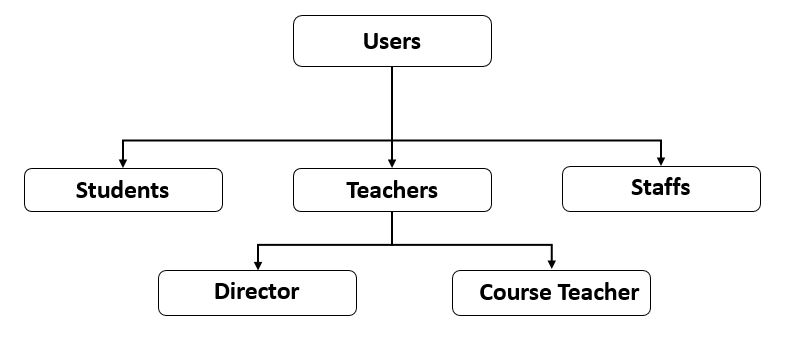
\includegraphics[width=10cm]{2.JPG}
    \caption{type of users}
    \label{fig:type of users}
\end{figure}

\section{Product Functions}
"IICT WEBSITE" store all the results of the students of program PGD, MIT. Also others programs can be included if necessary.
\begin{figure}[h!]
    \centering
    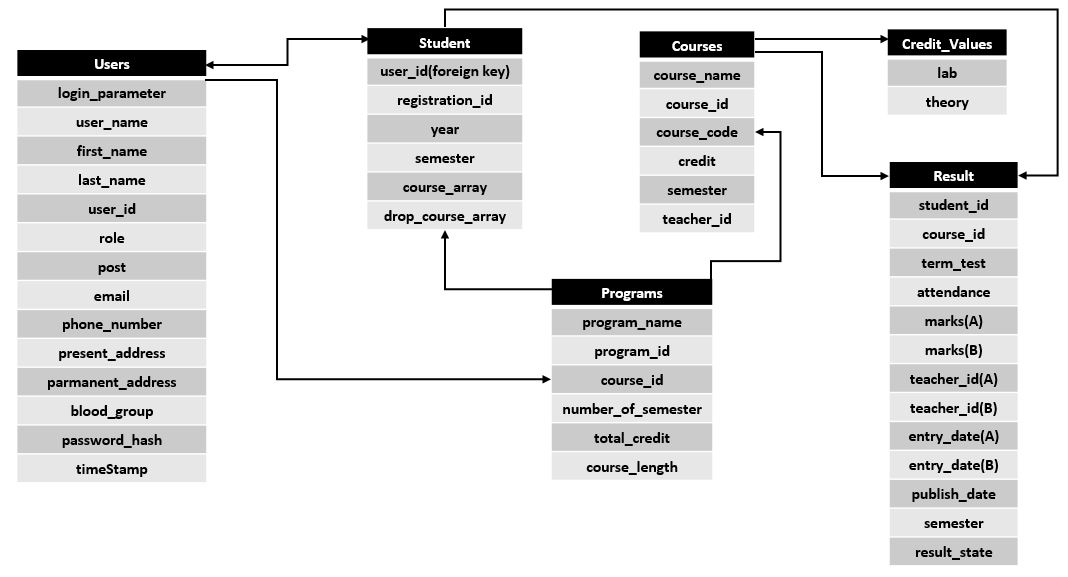
\includegraphics[width=15cm]{3.JPG}
    \caption{Data Flow Diagram}
    \label{fig:Data Flow Diagram}
\end{figure}
Before using the main function of the software result process, users have to be registered. 
\newline
All users have - login\_parameter, user\_name, first\_name, last\_name, user\_id, role, post, email, phone\_number, present\_address, parmanent\_address, blood\_group, password\_hash and timeStamp.
\newline
Students have some extra informations after complete his/her registration , such as - user\_id(foreign key), registration\_id, year, semester, course\_array and drop\_course\_array. These are the information that contains his/her result of his taken courses and program.
\newline
Each programs has some data - program\_name, program\_id, course\_id, nunmber\_of\_semester, total\_credit and course\_length. There will be onew or many course\_id in each programs.
\newline
Courses table contains - course\_name, course\_id, course\_code, credit, semester and teacher\_id.
\newline
Every course has its own Credit Values. Those have been 2 types - lab, theory.
\newline
Result is the main feature of all. It contains the values of all the exams of a particular student. It has data field - student\_id, course\_id, term\_test, attendance, marks(A), marks(B), teacher\_id(A), teacher\_id(B), entry\_date(A), entry\_date(B), publish\_date, semester	and result\_state.

\section{Operating Environment}
The website will be operate in any Operating Environment - Mac, Windows, Linux etc. 

\section{Design}
Student activities have 3 steps -
\begin{itemize}
    \item From Fill Up Process
    \item Courses Payment
    \item Student Profile
\end{itemize}
Top selected Student first fill his/her form, bank payment. After verification, student pays for their selected courses. Then he can enter his profile. 
\newline
Every student profile contains his/her personal information, results, taken courses, dropped courses and notice.
\newline
Notice will contain all the news of IICT.

\begin{figure}[h!]
    \centering
    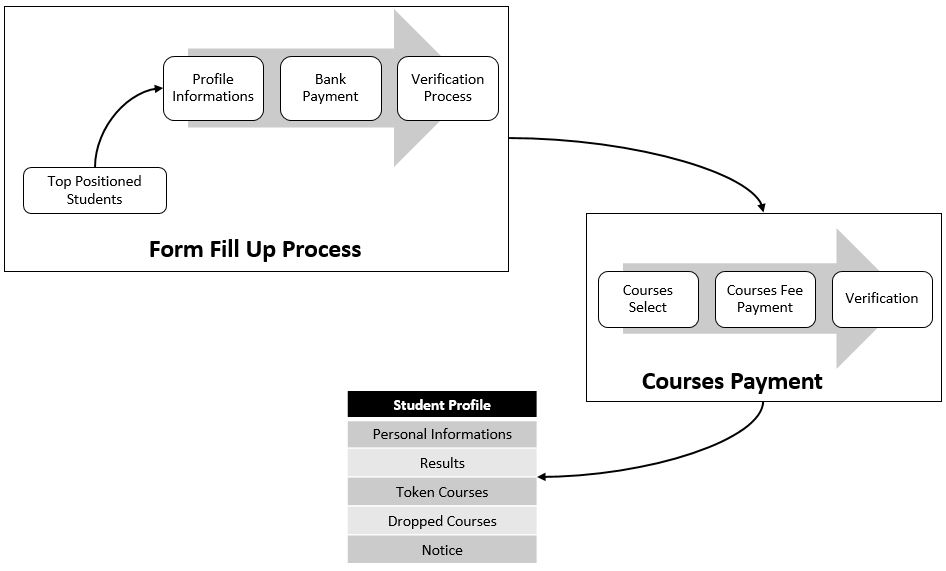
\includegraphics[width=15cm]{4.JPG}
    \caption{Student Activities}
    \label{fig:Students Activites}
\end{figure}
\newpage
Teacher activities have 2 steps - 
\begin{itemize}
    \item Director
    \item Course Teacher
\end{itemize}
Director can re-view the result, publish result, give notice and also create teacher. He can also perform course teacher activities.
\newline
Teacher creates results, view students and create notice.
\newline
\begin{figure}[h!]
    \centering
    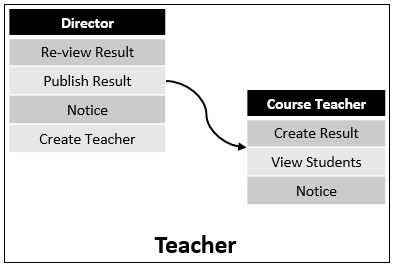
\includegraphics[width=10cm]{5.JPG}
    \caption{Teacher Activities}
    \label{fig:Teacher Activities}
\end{figure}
\newline
Staff has only one activity - 
\begin{itemize}
    \item Notice
\end{itemize} 
\begin{figure}[h!]
    \centering
    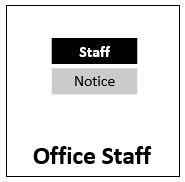
\includegraphics[width=5cm]{6.JPG}
    \caption{Staff Activities}
    \label{fig:Staff Activities}
\end{figure}

\chapter{External Interface Requirements}

\section{User Interfaces}
\lipsum[1-1]
\section{Hardware Interfaces}
\lipsum[1-1]
\section{Software Interfaces}
\lipsum[1-1]
\section{Communications Interfaces}
\lipsum[1-1]

\chapter{System Features}
"IICT WEBSITE" is a result processing web software. So the main art of this product is to enter data of results and publish. 

\section{Description and Priority}
"IICT WEBSITE" has features that are main and also some are sub. But all the feature is necessary for this software.
\newline
The features with priority up to down - 
\begin{enumerate}
    \item Result Creation : This is the goal feature of this software. It is been operated by teachers. They input the results of the students.
    \item Result Re-view : This is done by director.
    \item Result Publish : It is basically notice. This is mainly done by director or sometimes by staffs commanded by director.
    \item Teacher : Teacher takes the courses and create the results.
    \item Student : Student takes the courses of a program.
    \item Staff : Their only work is to post notice.
\end{enumerate}

\section{Functional Requirements}
The "IICT WEBSITE" website is being build on .NET framework, C\# language, React, React Redux, JavaScript and MongoDB.
\newline
Back-End - .NET framework, C\# language.
\newline
Font-End - React, React Redux, JavaScript.
\newline
Database -  MongoDB.


\chapter{Other Nonfunctional Requirements}

\section{Performance Requirements}
"IICT WEBSITE" will be used for result system of IICT programs, like - PGD, MIT. So for more interaction .NET, React and MongoDB is used. 

\section{Security Requirements}
No one without registered users can inter to the website. One particular user of a section only can perform his/her particular actions. 

\section{Software Quality Attributes}
In the development phase also testing and conferences of users is been continued. So that the quality of the software is been maintained and all the requirements are been fulfilled.
\newline
Database, logical and also UI test is required. 

\section{Business Rules}
"IICT WEBSITE" is for storing students results and publish those results of particular programs.
\newline
Basically save working time and pressure. 


\chapter{Other Requirements}
"IICT WEBSITE" needs maintenance as it is a long process software. It will need re-factoring and further the requirements can be changed as the field is changing frequently. 

\addappendix


\end{document}